\documentclass[12pt]{beamer}\usepackage[]{graphicx}\usepackage[]{color}
%% maxwidth is the original width if it is less than linewidth
%% otherwise use linewidth (to make sure the graphics do not exceed the margin)
\makeatletter
\def\maxwidth{ %
  \ifdim\Gin@nat@width>\linewidth
    \linewidth
  \else
    \Gin@nat@width
  \fi
}
\makeatother

\definecolor{fgcolor}{rgb}{0.345, 0.345, 0.345}
\newcommand{\hlnum}[1]{\textcolor[rgb]{0.686,0.059,0.569}{#1}}%
\newcommand{\hlstr}[1]{\textcolor[rgb]{0.192,0.494,0.8}{#1}}%
\newcommand{\hlcom}[1]{\textcolor[rgb]{0.678,0.584,0.686}{\textit{#1}}}%
\newcommand{\hlopt}[1]{\textcolor[rgb]{0,0,0}{#1}}%
\newcommand{\hlstd}[1]{\textcolor[rgb]{0.345,0.345,0.345}{#1}}%
\newcommand{\hlkwa}[1]{\textcolor[rgb]{0.161,0.373,0.58}{\textbf{#1}}}%
\newcommand{\hlkwb}[1]{\textcolor[rgb]{0.69,0.353,0.396}{#1}}%
\newcommand{\hlkwc}[1]{\textcolor[rgb]{0.333,0.667,0.333}{#1}}%
\newcommand{\hlkwd}[1]{\textcolor[rgb]{0.737,0.353,0.396}{\textbf{#1}}}%
\let\hlipl\hlkwb

\usepackage{framed}
\makeatletter
\newenvironment{kframe}{%
 \def\at@end@of@kframe{}%
 \ifinner\ifhmode%
  \def\at@end@of@kframe{\end{minipage}}%
  \begin{minipage}{\columnwidth}%
 \fi\fi%
 \def\FrameCommand##1{\hskip\@totalleftmargin \hskip-\fboxsep
 \colorbox{shadecolor}{##1}\hskip-\fboxsep
     % There is no \\@totalrightmargin, so:
     \hskip-\linewidth \hskip-\@totalleftmargin \hskip\columnwidth}%
 \MakeFramed {\advance\hsize-\width
   \@totalleftmargin\z@ \linewidth\hsize
   \@setminipage}}%
 {\par\unskip\endMakeFramed%
 \at@end@of@kframe}
\makeatother

\definecolor{shadecolor}{rgb}{.97, .97, .97}
\definecolor{messagecolor}{rgb}{0, 0, 0}
\definecolor{warningcolor}{rgb}{1, 0, 1}
\definecolor{errorcolor}{rgb}{1, 0, 0}
\newenvironment{knitrout}{}{} % an empty environment to be redefined in TeX

\usepackage{alltt}
\usepackage{tikz}

% make it pretty
% get rid of junk
\usetheme{default}
\usefonttheme[onlymath]{serif}
\beamertemplatenavigationsymbolsempty

% define a bunch of colors
\definecolor{offwhite}{RGB}{255,250,240}
\definecolor{gray}{RGB}{155,155,155}
\definecolor{foreground}{RGB}{80,80,80}
\definecolor{background}{RGB}{255,255,255}
%\definecolor{title}{RGB}{255,199,0}
\definecolor{title}{RGB}{89,132,212}
%\definecolor{subtitle}{RGB}{89,132,212}
\definecolor{subtitle}{RGB}{255,199,0}
\definecolor{hilit}{RGB}{248,117,79}
\definecolor{vhilit}{RGB}{255,111,207}
\definecolor{lolit}{RGB}{200,200,200}
\definecolor{lit}{RGB}{255,199,0}
\definecolor{mdlit}{RGB}{89,132,212}
\definecolor{link}{RGB}{248,117,79}

% a few color macros
\newcommand{\hilit}{\color{hilit}}
\newcommand{\vhilit}{\color{vhilit}}
\newcommand{\lit}{\color{lit}}
\newcommand{\mdlit}{\color{mdlit}}
\newcommand{\lolit}{\color{lolit}}

% use those colors
\setbeamercolor{titlelike}{fg=title}
\setbeamercolor{subtitle}{fg=subtitle}
\setbeamercolor{frametitle}{fg=gray}
%\setbeamercolor{structure}{fg=subtitle}
\setbeamercolor{structure}{fg=title}
\setbeamercolor{institute}{fg=lolit}
\setbeamercolor{normal text}{fg=foreground,bg=background}
\setbeamertemplate{itemize subitem}{{\textendash}}
\setbeamerfont{itemize/enumerate subbody}{size=\small}
\setbeamerfont{itemize/enumerate subitem}{size=\small}

% center title of slides
\setbeamertemplate{blocks}[rounded]
\setbeamertemplate{frametitle}[default][center]

% page number
\setbeamerfont{page number in foot}{size=\footnotesize}
\setbeamertemplate{footline}[frame number]

% default link color
\hypersetup{colorlinks, urlcolor={link}}

% a few macros
\newcommand{\code}[1]{\texttt{#1}}
\newcommand{\hicode}[1]{{\hilit \texttt{#1}}}
\newcommand{\locode}[1]{{\lolit \texttt{#1}}}
\newcommand{\bb}[1]{\begin{block}{#1}}
\newcommand{\eb}{\end{block}}
\newcommand{\bi}{\begin{itemize}}
\newcommand{\bbi}{\vspace{4pt} \begin{itemize} \itemsep8pt}
\newcommand{\ei}{\end{itemize}}
\newcommand{\bv}{\begin{verbatim}}
\newcommand{\ev}{\end{verbatim}}
\newcommand{\ig}{\includegraphics}
\newcommand{\subt}[1]{{\footnotesize \color{subtitle} {#1}}}
\newcommand{\ttsm}{\tt \small}
\newcommand{\ttfn}{\tt \footnotesize}
\newcommand{\figh}[2]{\centerline{\includegraphics[height=#2\textheight]{#1}}}
\newcommand{\figw}[2]{\centerline{\includegraphics[width=#2\textwidth]{#1}}}



%------------------------------------------------

\title{Statistical Operations and Matrices (II)}
\subtitle{Predictive Modeling \& Statistical Learning}
\author{\href{http://www.gastonsanchez.com}{Gaston Sanchez}}
\institute{\href{https://creativecommons.org/licenses/by-sa/4.0/}{\tt \scriptsize \color{foreground} CC BY-SA 4.0}}
\date{}
\IfFileExists{upquote.sty}{\usepackage{upquote}}{}
\begin{document}



% no page number in first slide
{
  \setbeamertemplate{footline}{} 
  \frame{\titlepage} 
}

%------------------------------------------------

\begin{frame}
\begin{center}
\Huge{\hilit{Geometry of the Data Matrix}}
\end{center}
\end{frame}

%------------------------------------------------

\begin{frame}
\frametitle{Matrix Structure}

\begin{block}{Data}
The analyzed data can be expressed in matrix format $\mathbf{X}$:

\[ \underset{n \times p}{\mathbf{X}} = 
\left[\begin{array}{cccc}
x_{11} & x_{12} & \cdots & x_{1p} \\
x_{21} & x_{22} & \cdots & x_{2p} \\
\vdots & \vdots & \ddots & \vdots \\
x_{n1} & x_{n2} & \cdots & x_{np} \\
\end{array}\right]
\]
\end{block}

\begin{itemize}
 \item $n$ objects in the rows
 \item $p$ quantitative variables in the columns
\end{itemize}

\end{frame}

%------------------------------------------------

\begin{frame}
\begin{center}
\Huge{\hilit{Looking at Rows \\ and Columns}}
\end{center}
\end{frame}

%------------------------------------------------

\begin{frame}
\frametitle{Data Concerns}

\begin{columns}[t]
\begin{column}{0.1\textwidth}
%--- empty space ---%
\end{column}

\begin{column}{0.8\textwidth}
\bb{Two sides of the same coin}
When the analyzed data can be expressed as a matrix with objects in rows, and variables in columns, we commonly care for two issues:
\bi
 \item Study the {\hilit resemblance between objects}
 \item Study the {\hilit relationships among variables}
\ei
\eb
\end{column}

\begin{column}{0.1\textwidth}
%--- empty space ---%
\end{column}
\end{columns}

\end{frame}

%------------------------------------------------

\begin{frame}
\frametitle{Data Perspectives}
\begin{center}
\ig[width=10cm]{images/duality_data_matrix.pdf}
\end{center}
\end{frame}

%------------------------------------------------

\begin{frame}
\frametitle{Objects Perspective}
\begin{center}
\ig[width=11cm]{images/duality_column_space.pdf}
\end{center}
\end{frame}

%------------------------------------------------

\begin{frame}
\frametitle{}
\begin{center}
\ig[width=11cm]{images/duality_objects_cloud.pdf}
\end{center}
\end{frame}

%------------------------------------------------

\begin{frame}
\frametitle{Variables Perspective}
\begin{center}
\ig[width=11cm]{images/duality_row_space.pdf}
\end{center}
\end{frame}

%------------------------------------------------

\begin{frame}
\frametitle{}
\begin{center}
\ig[width=11cm]{images/duality_variables_cloud.pdf}
\end{center}
\end{frame}

%------------------------------------------------

\begin{frame}
\begin{center}
\Huge{\hilit{Raw Data}}
\end{center}
\end{frame}

%------------------------------------------------

\begin{frame}
\frametitle{Raw Data Matrix}

The analyzed data can be expressed in matrix format $\mathbf{X}$:

\[ \underset{n \times p}{\mathbf{X}} = 
\left[\begin{array}{cccc}
x_{11} & x_{12} & \cdots & x_{1p} \\
x_{21} & x_{22} & \cdots & x_{2p} \\
\vdots & \vdots & \ddots & \vdots \\
x_{n1} & x_{n2} & \cdots & x_{np} \\
\end{array}\right]
\]

\begin{itemize}
 \item $n$ objects in the rows
 \item $p$ quantitative variables in the columns
\end{itemize}

\end{frame}

%------------------------------------------------

\begin{frame}[fragile]
\frametitle{Data set \code{mtcars}}

First 10 rows:
\begin{knitrout}\scriptsize
\definecolor{shadecolor}{rgb}{0.969, 0.969, 0.969}\color{fgcolor}\begin{kframe}
\begin{verbatim}
                   mpg cyl  disp  hp drat    wt  qsec vs am gear carb
Mazda RX4         21.0   6 160.0 110 3.90 2.620 16.46  0  1    4    4
Mazda RX4 Wag     21.0   6 160.0 110 3.90 2.875 17.02  0  1    4    4
Datsun 710        22.8   4 108.0  93 3.85 2.320 18.61  1  1    4    1
Hornet 4 Drive    21.4   6 258.0 110 3.08 3.215 19.44  1  0    3    1
Hornet Sportabout 18.7   8 360.0 175 3.15 3.440 17.02  0  0    3    2
Valiant           18.1   6 225.0 105 2.76 3.460 20.22  1  0    3    1
Duster 360        14.3   8 360.0 245 3.21 3.570 15.84  0  0    3    4
Merc 240D         24.4   4 146.7  62 3.69 3.190 20.00  1  0    4    2
Merc 230          22.8   4 140.8  95 3.92 3.150 22.90  1  0    4    2
Merc 280          19.2   6 167.6 123 3.92 3.440 18.30  1  0    4    4
\end{verbatim}
\end{kframe}
\end{knitrout}

Let's use variables: \code{mpg}, \code{disp}, \code{hp}, and \code{wt}.

\end{frame}

%------------------------------------------------

\begin{frame}[fragile]



\begin{knitrout}\footnotesize
\definecolor{shadecolor}{rgb}{0.969, 0.969, 0.969}\color{fgcolor}

{\centering 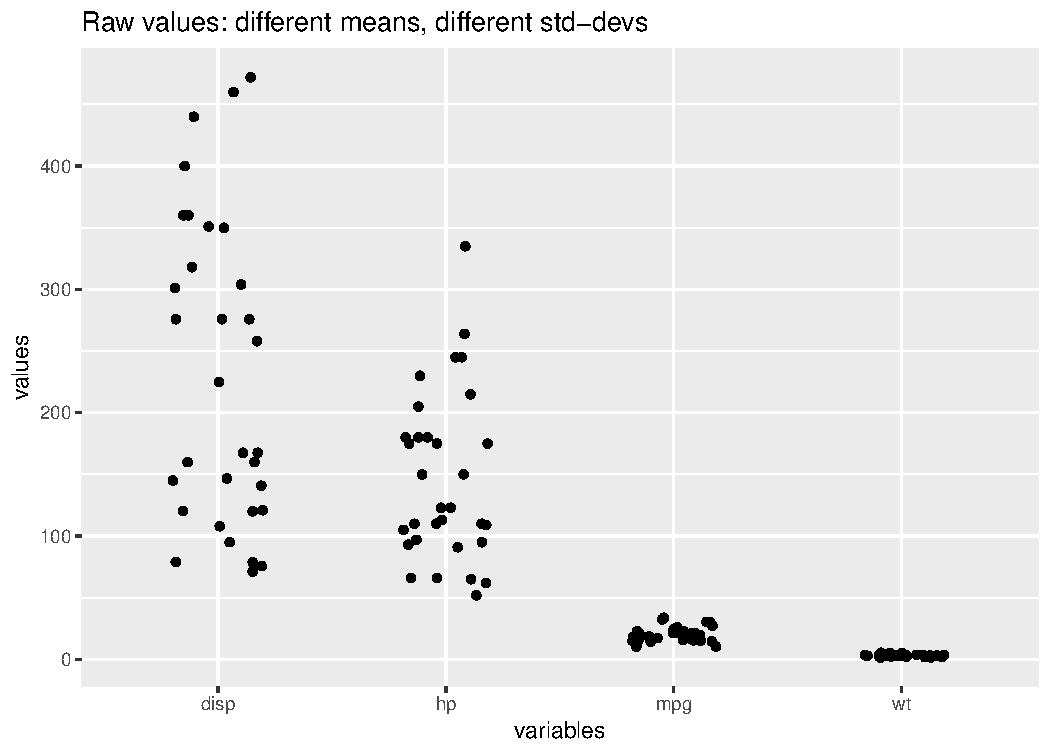
\includegraphics[width=\maxwidth]{figure/unnamed-chunk-2-1} 

}



\end{knitrout}

\end{frame}

%------------------------------------------------

\begin{frame}[fragile]

\begin{knitrout}\footnotesize
\definecolor{shadecolor}{rgb}{0.969, 0.969, 0.969}\color{fgcolor}

{\centering 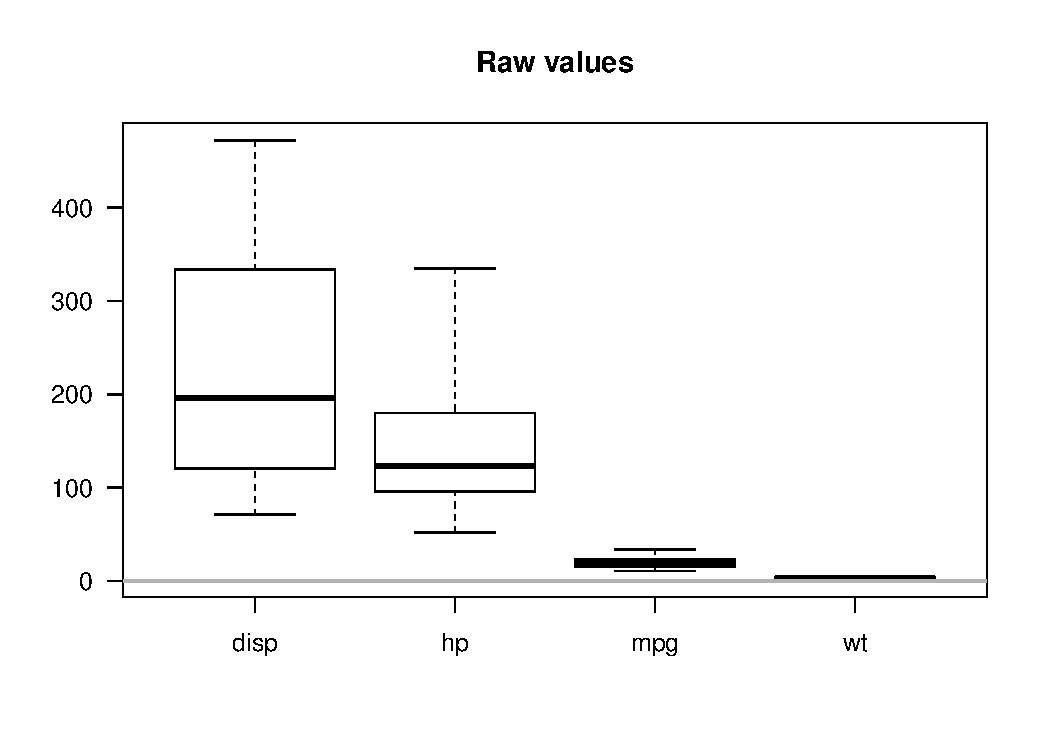
\includegraphics[width=\maxwidth]{figure/unnamed-chunk-3-1} 

}



\end{knitrout}

\end{frame}

%------------------------------------------------

\begin{frame}
\begin{center}
\Huge{\hilit{Centering Data Matrix}}
\end{center}
\end{frame}

%------------------------------------------------

\begin{frame}
\frametitle{Mean-Centered Data Matrix}

A common operation consists of {\hilit \textbf{centering}} the data, which involves
mean-centering the variables so that they all have mean zero.

\end{frame}

%------------------------------------------------

\begin{frame}
\frametitle{Mean-Centered Data Matrix}

The mean-centered (a.k.a. column centered) matrix $\mathbf{X_C}$:

\[ \underset{n \times p}{\mathbf{X_C}} = 
\left[\begin{array}{cccc}
x_{11} - \bar{x}_1 & x_{12} - \bar{x}_2 & \cdots & x_{1p} - \bar{x}_p \\
x_{21} - \bar{x}_1 & x_{22} - \bar{x}_2 & \cdots & x_{2p} - \bar{x}_p \\
\vdots & \vdots & \ddots & \vdots \\
x_{n1} - \bar{x}_1 & x_{n2} - \bar{x}_2 & \cdots & x_{np} - \bar{x}_p \\
\end{array}\right]
\]

where $\bar{x}_j$ is the mean of the $j$-th variable ($j = 1, \dots, p$)

\end{frame}

%------------------------------------------------

\begin{frame}
\frametitle{Mean-Centered Data Matrix}

Using matrix notation, the centering operation is expressed as:

$$
\mathbf{X_C} = (\mathbf{I} - \frac{1}{n} \mathbf{11^\mathsf{T}}) \mathbf{X} 
$$

\bi
  \item $\mathbf{I}$ is the $n \times n$ identity matrix
  \item $\mathbf{1}$ is an $n \times 1$ vector of ones
\ei

\bigskip
{\mdlit $\mathbf{I} - \frac{1}{n} \mathbf{11^\mathsf{T}}$} is sometimes called the 
{\mdlit \textit{centering}} operator

\end{frame}

%------------------------------------------------

\begin{frame}
\frametitle{Centering Effects}

{\large What does mean-centering do to the cloud of points?}

\end{frame}

%------------------------------------------------

\begin{frame}[fragile]



\begin{knitrout}\footnotesize
\definecolor{shadecolor}{rgb}{0.969, 0.969, 0.969}\color{fgcolor}

{\centering 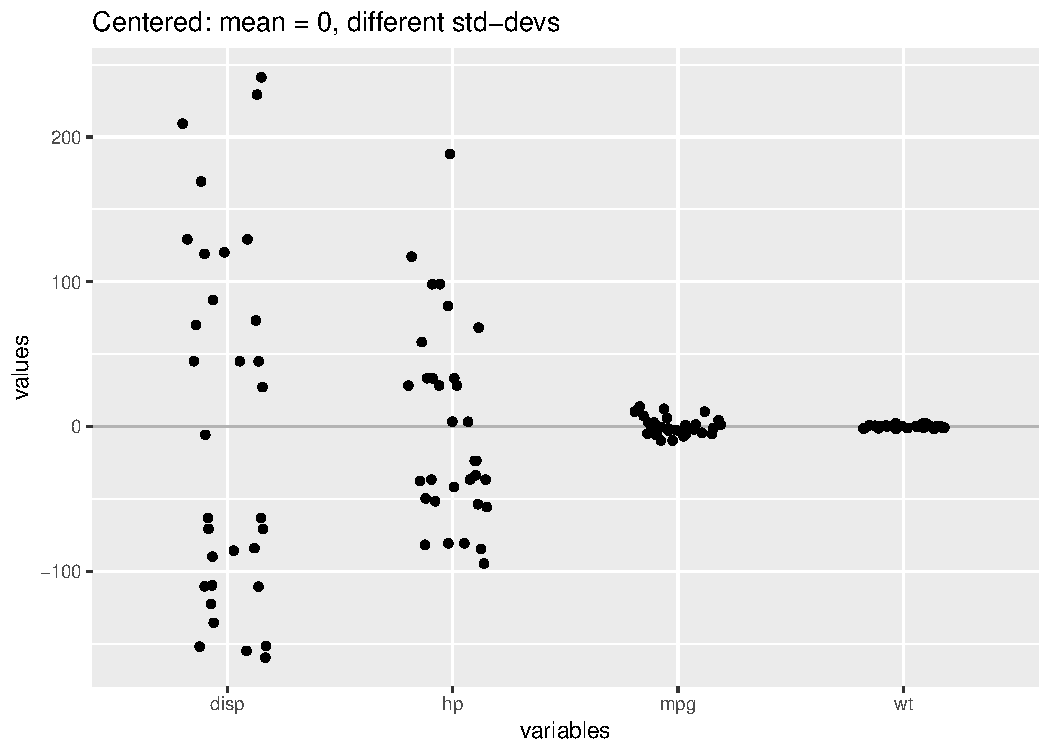
\includegraphics[width=\maxwidth]{figure/unnamed-chunk-5-1} 

}



\end{knitrout}

\end{frame}

%------------------------------------------------

\begin{frame}[fragile]

\begin{knitrout}\footnotesize
\definecolor{shadecolor}{rgb}{0.969, 0.969, 0.969}\color{fgcolor}

{\centering 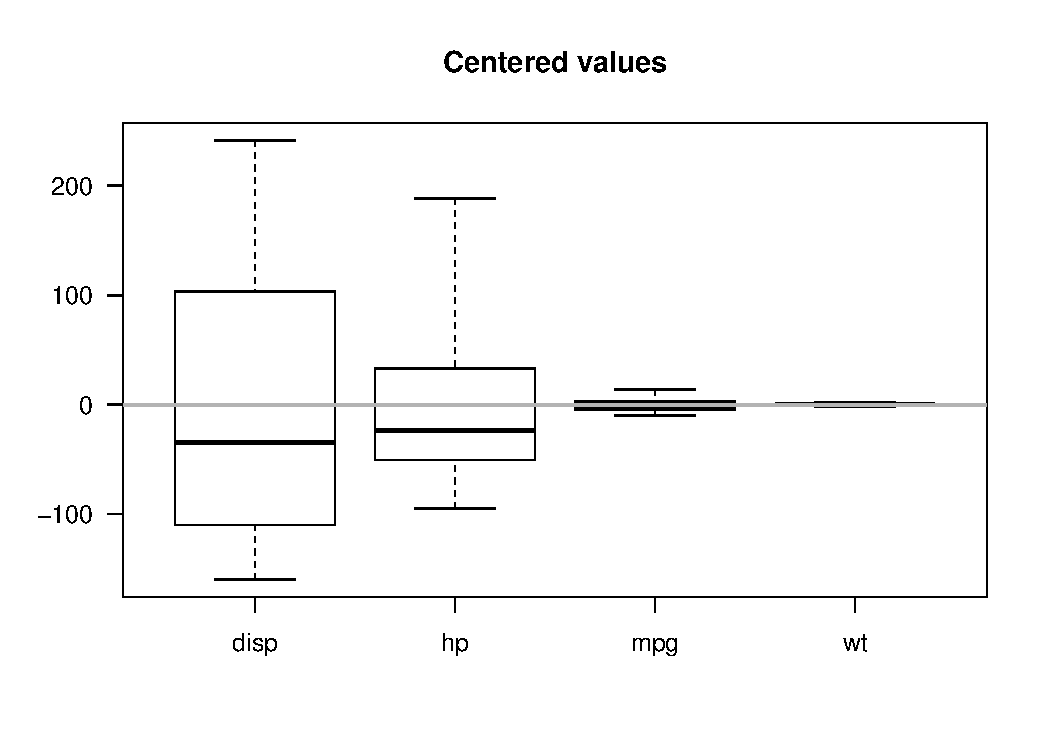
\includegraphics[width=\maxwidth]{figure/unnamed-chunk-6-1} 

}



\end{knitrout}

\end{frame}

%------------------------------------------------

\begin{frame}[fragile]
\frametitle{Centering Matrices in R}

Centering with \code{scale()}

\begin{knitrout}\footnotesize
\definecolor{shadecolor}{rgb}{0.969, 0.969, 0.969}\color{fgcolor}\begin{kframe}
\begin{alltt}
\hlstd{X_centered} \hlkwb{<-} \hlkwd{scale}\hlstd{(X,} \hlkwc{center} \hlstd{=} \hlnum{TRUE}\hlstd{,} \hlkwc{scale} \hlstd{=} \hlnum{FALSE}\hlstd{)}
\end{alltt}
\end{kframe}
\end{knitrout}

Or also like this:
\begin{knitrout}\footnotesize
\definecolor{shadecolor}{rgb}{0.969, 0.969, 0.969}\color{fgcolor}\begin{kframe}
\begin{alltt}
\hlstd{centroid} \hlkwb{<-} \hlkwd{colMeans}\hlstd{(X)}
\hlstd{X_centered} \hlkwb{<-} \hlkwd{sweep}\hlstd{(X,} \hlnum{2}\hlstd{, centroid,} \hlkwc{FUN} \hlstd{=} \hlstr{"-"}\hlstd{)}
\end{alltt}
\end{kframe}
\end{knitrout}

\end{frame}

%------------------------------------------------

\begin{frame}
\frametitle{Cloud of individuals}
\begin{center}
\ig[height=7cm]{images/cloud_obs_centering1.pdf}

{\lolit Raw (i.e. non-centered) variables}
\end{center}
\end{frame}

%------------------------------------------------

\begin{frame}
\frametitle{Cloud of individuals}
\begin{center}
\ig[height=7cm]{images/cloud_obs_centering2.pdf}

{\lolit Centered variables}
\end{center}
\end{frame}

%------------------------------------------------

\begin{frame}
\begin{center}
\Huge{\hilit{Scaled Data Matrix}}
\end{center}
\end{frame}

%------------------------------------------------

\begin{frame}
\frametitle{Scaled or Normalized Data Matrix}

The scaled or \textit{Normalized} matrix $\mathbf{X_N}$:

\[ \underset{n \times p}{\mathbf{X_N}} = 
\left[\begin{array}{cccc}
a_1 x_{11} & a_2 x_{12} & \cdots & a_p x_{1p} \\
a_1 x_{21} & a_2 x_{22} & \cdots & a_p x_{2p} \\
\vdots & \vdots & \ddots & \vdots \\
a_1 x_{n1} & a_2 x_{n2} & \cdots & a_p x_{np} \\
\end{array}\right]
\]

where $a_j$ is a scaling factor for the $j$-th column

\end{frame}

%------------------------------------------------

\begin{frame}
\frametitle{Some Scaling Options}

Probably the most common scaling option is to divide by the standard deviation:

$$
a_j = \frac{1}{sd_j} = 1 / \sqrt{\frac{1}{n-1} \sum_{i=1}^{n} (x_{ij} - \bar{x}_j)^2}
$$

\end{frame}

%------------------------------------------------

\begin{frame}[fragile]
\frametitle{Scaling Matrices in R}

Scaling with standard deviation

\begin{knitrout}\footnotesize
\definecolor{shadecolor}{rgb}{0.969, 0.969, 0.969}\color{fgcolor}\begin{kframe}
\begin{alltt}
\hlstd{stdevs} \hlkwb{<-} \hlkwd{apply}\hlstd{(X,} \hlnum{2}\hlstd{, sd)}

\hlstd{X_scaled} \hlkwb{<-} \hlkwd{scale}\hlstd{(X,} \hlkwc{center} \hlstd{=} \hlnum{FALSE}\hlstd{,} \hlkwc{scale} \hlstd{= stdevs)}
\end{alltt}
\end{kframe}
\end{knitrout}

\end{frame}

%------------------------------------------------

\begin{frame}[fragile]



\begin{knitrout}\footnotesize
\definecolor{shadecolor}{rgb}{0.969, 0.969, 0.969}\color{fgcolor}

{\centering 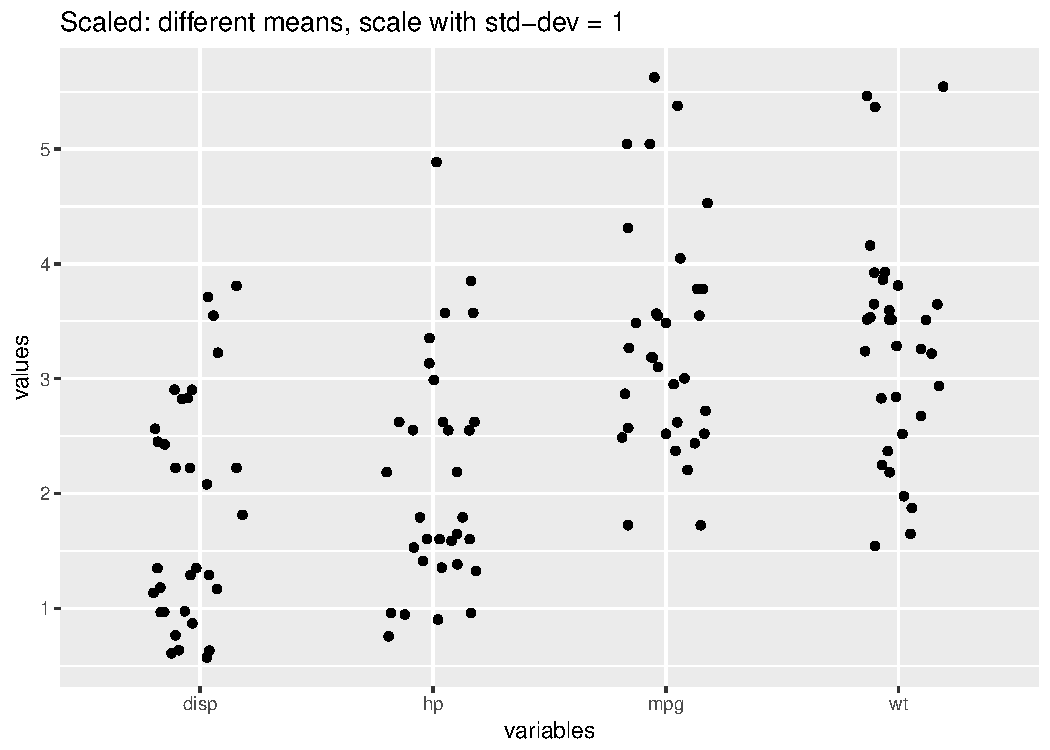
\includegraphics[width=\maxwidth]{figure/unnamed-chunk-11-1} 

}



\end{knitrout}

\end{frame}

%------------------------------------------------

\begin{frame}[fragile]

\begin{knitrout}\footnotesize
\definecolor{shadecolor}{rgb}{0.969, 0.969, 0.969}\color{fgcolor}

{\centering 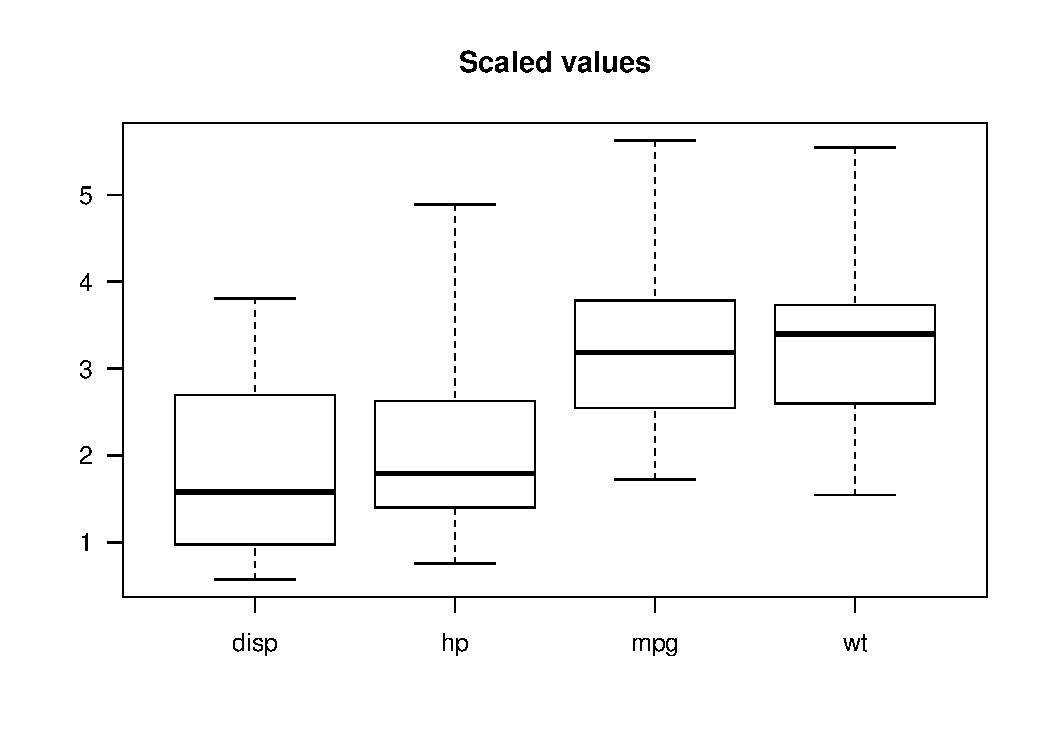
\includegraphics[width=\maxwidth]{figure/unnamed-chunk-12-1} 

}



\end{knitrout}

\end{frame}

%------------------------------------------------

\begin{frame}
\frametitle{Some Scaling Options}

Other typical scaling options are based on $L_p$-norms:
$$
L_p\text{-norm = } \left ( \sum_{i=1}^{n} |x_{ij}|^p \right )^{1/p}
$$

\bigskip
The most common $L_p$-norms are:
\bbi
  \item $L_1$-norm: $\sum_{i=1}^{n} | x_{ij} |$
  \item $L_2$-norm: $\sqrt{\sum_{i=1}^{n} (x_{ij})^2}$
  \item $L_{\infty}$-norm: $max \{ |x_{i1}|, \dots, |x_{ip}| \}$
\ei

\end{frame}

%------------------------------------------------

\begin{frame}
\frametitle{Some Scaling Options}

Using $L_p$-norms, the scaling factors $a_j$ are:

\bbi
  \item $L_1$-norm: $\quad a_j = 1 / \sum_{i=1}^{n} | x_{ij} |$
  \item $L_2$-norm: $\quad a_j = 1 / \sqrt{\sum_{i=1}^{n} (x_{ij})^2}$
  \item $L_{\infty}$-norm: $\quad a_j = 1 / max \{ |x_{i1}|, \dots, |x_{ip}| \}$
  \item $L_p$-norm: $\quad a_j = 1 / \left ( \sum_{i=1}^{n} |x_{ij}|^p \right )^{1/p}$
\ei

\end{frame}

%------------------------------------------------

\begin{frame}
\frametitle{Scaled or Normalized Data Matrix}

The scaling factors $a_j$ can be put in a diagonal matrix $\mathbf{D_a}$

\[ \underset{p \times p}{\mathbf{D_a}} = 
\left[\begin{array}{cccc}
a_1 & 0   & \cdots & 0 \\
0   & a_2 & \cdots & 0 \\
\vdots & \vdots & \ddots & \vdots \\
0   & 0   & \cdots & a_p \\
\end{array}\right]
\]

then the scaled or normalized data matrix is given by:

{\large
$$
\mathbf{X_N} = \mathbf{X D_a}
$$
}

\end{frame}

%------------------------------------------------

\begin{frame}
\frametitle{Normalizing Effects}

What does normalizing (i.e. scaling) do to the cloud of points?

\end{frame}

%------------------------------------------------

\begin{frame}[fragile]
\frametitle{Scaling Matrices in R}

Scaling with $L_1$-norm:

$$
\sum_{i=1}^{n} | x_{ij} |
$$

\begin{knitrout}\footnotesize
\definecolor{shadecolor}{rgb}{0.969, 0.969, 0.969}\color{fgcolor}\begin{kframe}
\begin{alltt}
\hlcom{# L-1 norm}
\hlstd{one_norms} \hlkwb{<-} \hlkwd{apply}\hlstd{(X,} \hlnum{2}\hlstd{,} \hlkwa{function}\hlstd{(}\hlkwc{u}\hlstd{)} \hlkwd{sum}\hlstd{(}\hlkwd{abs}\hlstd{(u)))}

\hlstd{X_scaled} \hlkwb{<-} \hlkwd{scale}\hlstd{(X,} \hlkwc{center} \hlstd{=} \hlnum{FALSE}\hlstd{,} \hlkwc{scale} \hlstd{= one_norms)}
\end{alltt}
\end{kframe}
\end{knitrout}

\end{frame}

%------------------------------------------------

\begin{frame}[fragile]



\begin{knitrout}\footnotesize
\definecolor{shadecolor}{rgb}{0.969, 0.969, 0.969}\color{fgcolor}

{\centering 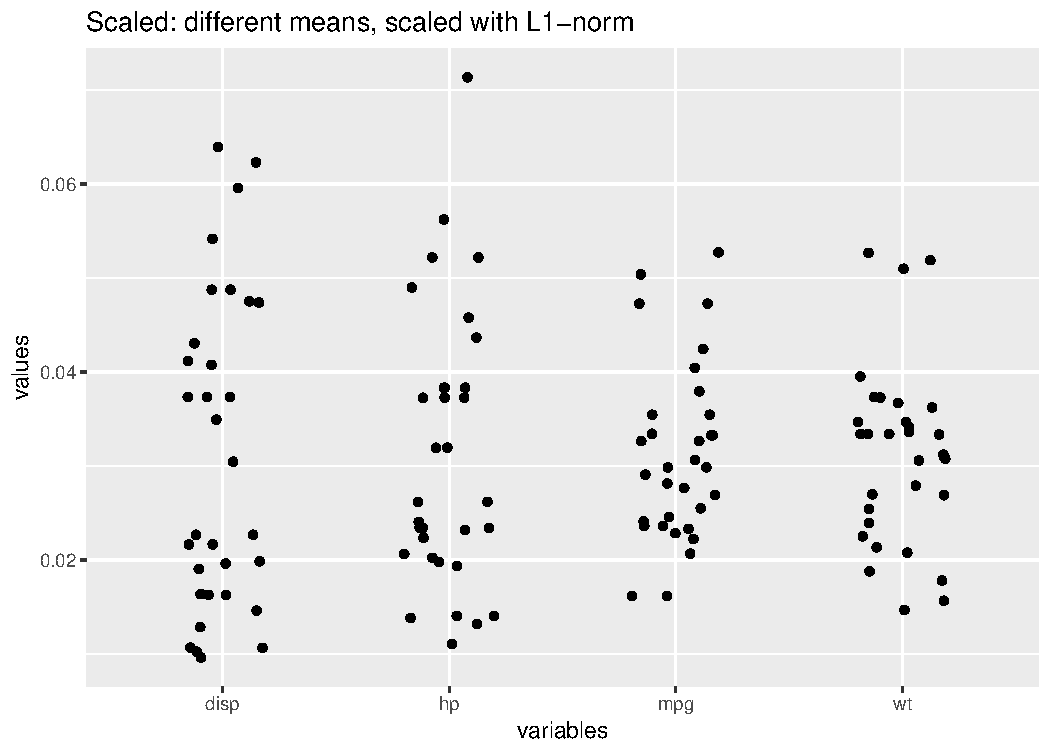
\includegraphics[width=\maxwidth]{figure/unnamed-chunk-15-1} 

}



\end{knitrout}

\end{frame}

%------------------------------------------------

\begin{frame}[fragile]
\frametitle{Scaling in R examples}

Scaling with $L_2$-norm

$$
\sqrt{\sum_{i=1}^{n} (x_{ij})^2}
$$

\begin{knitrout}\footnotesize
\definecolor{shadecolor}{rgb}{0.969, 0.969, 0.969}\color{fgcolor}\begin{kframe}
\begin{alltt}
\hlcom{# L-2 norm}
\hlstd{two_norms} \hlkwb{<-} \hlkwd{apply}\hlstd{(X,} \hlnum{2}\hlstd{,} \hlkwa{function}\hlstd{(}\hlkwc{u}\hlstd{)} \hlkwd{sqrt}\hlstd{(}\hlkwd{sum}\hlstd{(u}\hlopt{*}\hlstd{u)))}

\hlstd{X_scaled} \hlkwb{<-} \hlkwd{scale}\hlstd{(X,} \hlkwc{center} \hlstd{=} \hlnum{FALSE}\hlstd{,} \hlkwc{scale} \hlstd{= two_norms)}
\end{alltt}
\end{kframe}
\end{knitrout}

\end{frame}

%------------------------------------------------

\begin{frame}[fragile]



\begin{knitrout}\footnotesize
\definecolor{shadecolor}{rgb}{0.969, 0.969, 0.969}\color{fgcolor}

{\centering 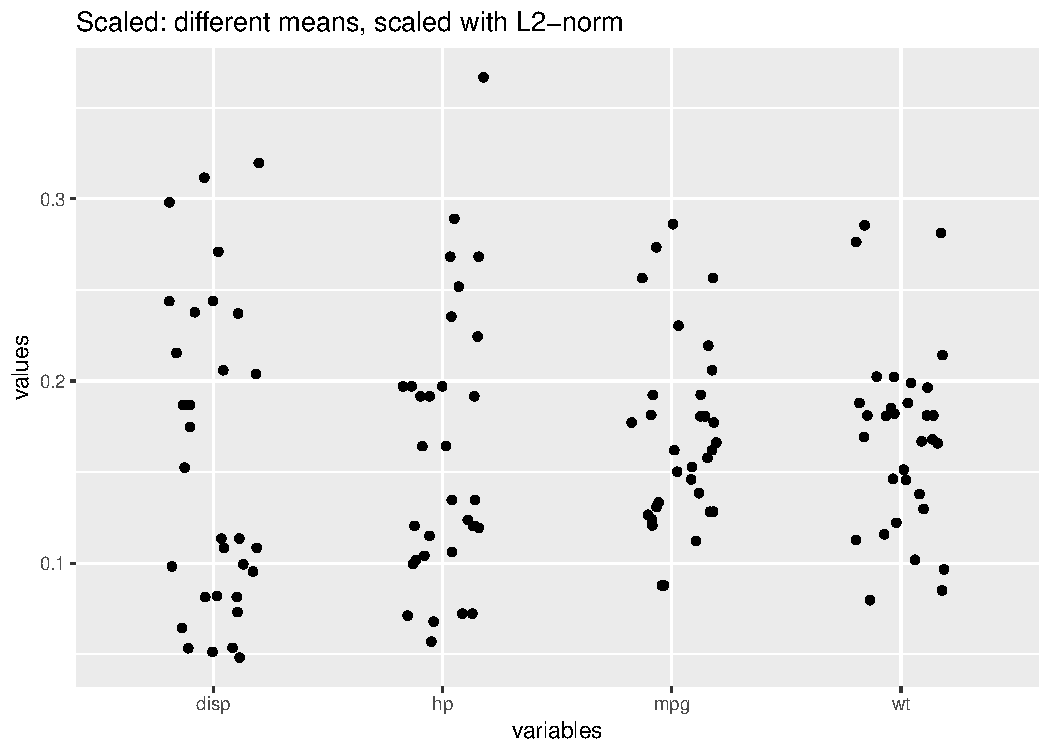
\includegraphics[width=\maxwidth]{figure/unnamed-chunk-18-1} 

}



\end{knitrout}

\end{frame}

%------------------------------------------------

\begin{frame}[fragile]
\frametitle{Scaling Matrices in R}

Scaling with $L_{\infty}$-norm
$$
max \{ |x_{i1}|, \dots, |x_{ip}| \}
$$

\begin{knitrout}\footnotesize
\definecolor{shadecolor}{rgb}{0.969, 0.969, 0.969}\color{fgcolor}\begin{kframe}
\begin{alltt}
\hlcom{# L-inf norm}
\hlstd{inf_norms} \hlkwb{<-} \hlkwd{apply}\hlstd{(X,} \hlnum{2}\hlstd{,} \hlkwa{function}\hlstd{(}\hlkwc{u}\hlstd{)} \hlkwd{max}\hlstd{(}\hlkwd{abs}\hlstd{(u)))}

\hlstd{X_scaled} \hlkwb{<-} \hlkwd{scale}\hlstd{(X,} \hlkwc{center} \hlstd{=} \hlnum{FALSE}\hlstd{,} \hlkwc{scale} \hlstd{= inf_norms)}
\end{alltt}
\end{kframe}
\end{knitrout}

\end{frame}

%------------------------------------------------

\begin{frame}[fragile]



\begin{knitrout}\footnotesize
\definecolor{shadecolor}{rgb}{0.969, 0.969, 0.969}\color{fgcolor}

{\centering 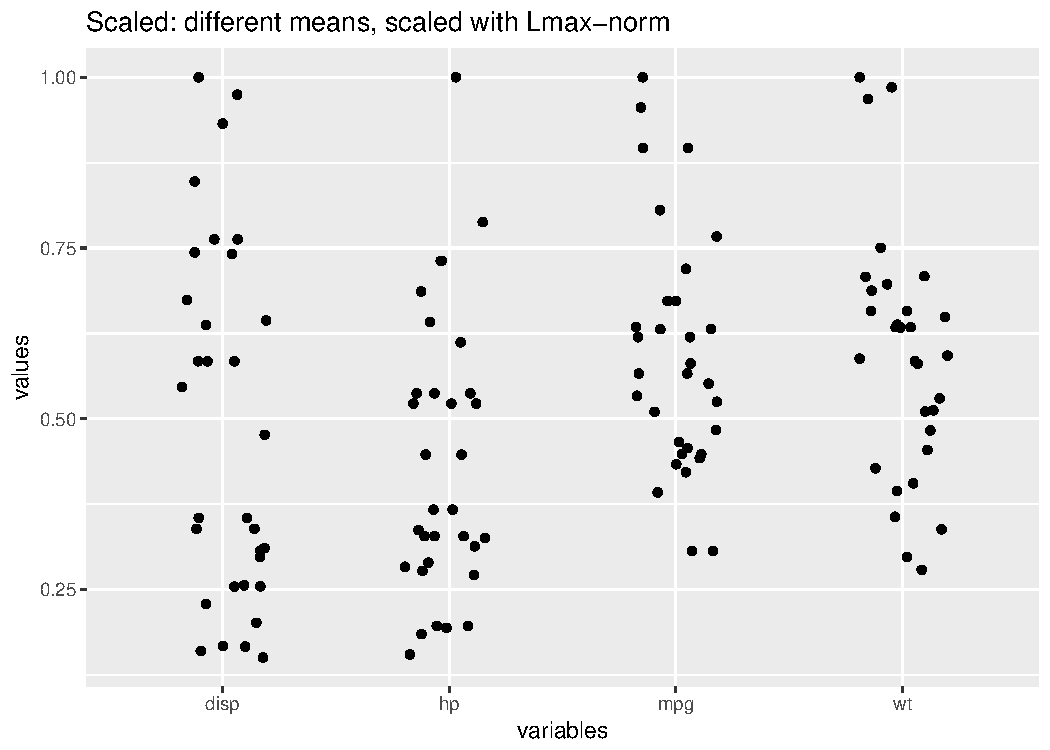
\includegraphics[width=\maxwidth]{figure/unnamed-chunk-21-1} 

}



\end{knitrout}

\end{frame}

%------------------------------------------------

\begin{frame}
\begin{center}
\Huge{\hilit{Standardized Data Matrix}}
\end{center}
\end{frame}

%------------------------------------------------

\begin{frame}
\frametitle{Standardized Data Matrix}

The standardized matrix $\mathbf{X_S}$ is the mean-centered and scaled 
(by the standard deviation) matrix:

\[ \underset{n \times p}{\mathbf{X_S}} = 
\left[\begin{array}{cccc}
\frac{x_{11} - \bar{x}_1}{sd_1} & \frac{x_{12} - \bar{x}_2}{sd_2} & \cdots & \frac{x_{1p} - \bar{x}_p}{sd_p} \\
\frac{x_{21} - \bar{x}_1}{sd_1} & \frac{x_{22} - \bar{x}_2}{sd_2} & \cdots & \frac{x_{2p} - \bar{x}_p}{sd_p} \\
\vdots & \vdots & \ddots & \vdots \\
\frac{x_{n1} - \bar{x}_1}{sd_1} & \frac{x_{n2} - \bar{x}_2}{sd_2} & \cdots & \frac{x_{np} - \bar{x}_p}{sd_p} \\
\end{array}\right]
\]

\bi
  \item $\bar{x}_j$ is the mean of the $j$-th variable
  \item $sd_j$ is the standard deviation of the $j$-th variable
\ei

\end{frame}

%------------------------------------------------

\begin{frame}[fragile]



\begin{knitrout}\footnotesize
\definecolor{shadecolor}{rgb}{0.969, 0.969, 0.969}\color{fgcolor}

{\centering 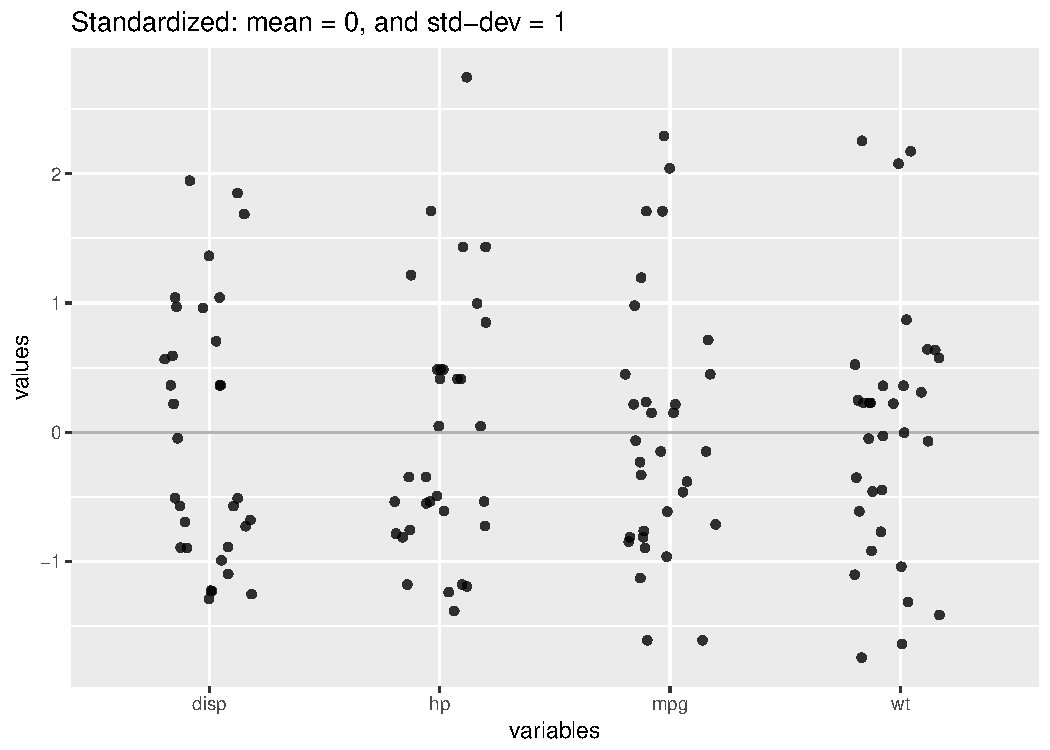
\includegraphics[width=\maxwidth]{figure/unnamed-chunk-23-1} 

}



\end{knitrout}

\end{frame}

%------------------------------------------------

\begin{frame}[fragile]

\begin{knitrout}\footnotesize
\definecolor{shadecolor}{rgb}{0.969, 0.969, 0.969}\color{fgcolor}

{\centering 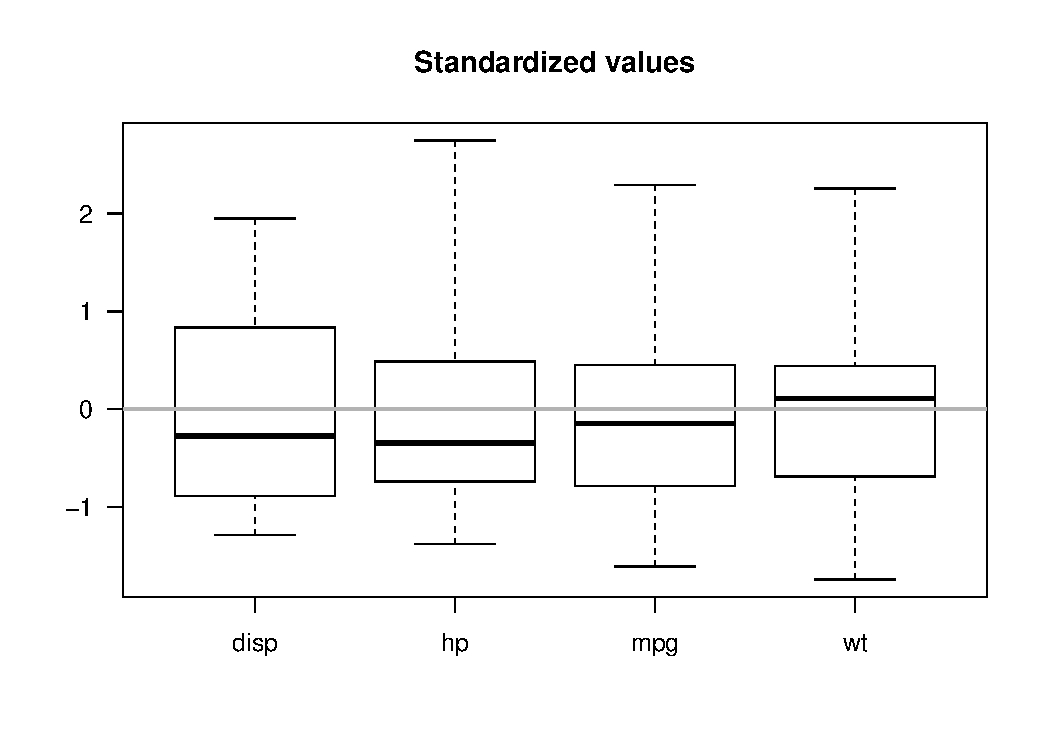
\includegraphics[width=\maxwidth]{figure/unnamed-chunk-24-1} 

}



\end{knitrout}

\end{frame}

%------------------------------------------------

\begin{frame}
\frametitle{Standardized Data Matrix}

When the scaling factors $a_j$ are the standard deviations $sd_j$, 
the scaling matrix $\mathbf{D}_{\frac{1}{sd}}$ is:

\[ \underset{p \times p}{\mathbf{D}_{\frac{1}{sd}}} = 
\left[\begin{array}{cccc}
\frac{1}{sd_1} & 0 & \cdots & 0 \\
0 & \frac{1}{sd_2} & \cdots & 0 \\
\vdots & \vdots & \ddots & \vdots \\
0 & 0 & \cdots & \frac{1}{sd_p} \\
\end{array}\right]
\]

then the standardized data matrix $\mathbf{X_S}$
$$
\mathbf{X_S} = \mathbf{X_C} \mathbf{D}_{\frac{1}{sd}} = (\mathbf{I} - \frac{1}{n} \mathbf{11^\mathsf{T}}) \mathbf{X} \mathbf{D}_{\frac{1}{sd}}
$$

\end{frame}

%------------------------------------------------

\begin{frame}[fragile]
\frametitle{Standardizing Matrices in R}

Standardizing with \code{scale()}

\begin{knitrout}\footnotesize
\definecolor{shadecolor}{rgb}{0.969, 0.969, 0.969}\color{fgcolor}\begin{kframe}
\begin{alltt}
\hlstd{X_std} \hlkwb{<-} \hlkwd{scale}\hlstd{(X,} \hlkwc{center} \hlstd{=} \hlnum{TRUE}\hlstd{,} \hlkwc{scale} \hlstd{=} \hlnum{TRUE}\hlstd{)}

\hlcom{# equivalent to}
\hlstd{X_std} \hlkwb{<-} \hlkwd{scale}\hlstd{(X)}
\end{alltt}
\end{kframe}
\end{knitrout}

\end{frame}

%------------------------------------------------

\begin{frame}
\begin{center}
\Huge{\hilit{Objects and their weights}}
\end{center}
\end{frame}

%------------------------------------------------

\begin{frame}
\frametitle{Weights of Objects}

\bi
  \item We can assume that each object is associated to a \textbf{weight}
  \item Think of a weight as the ``importance'' of an observation
  \item Usually, we assume equal weights $1/n$ (i.e. equal importance)
  \item If we assume that objects come from a random sample, then 
  the $n$ objects have the same chance $1/n$ of being selected
  \item Sometimes, however, it is convenient to assume that each object
  has a general weight $w_i > 0$, such that $\sum_{i=1}^{n} w_i = 1$
\ei

\end{frame}

%------------------------------------------------

\begin{frame}
\frametitle{Weights of Objects}

We can consider a diagonal matrix of object weights $\mathbf{D}$:

\[ \underset{n \times p}{\mathbf{D}} = 
\left[\begin{array}{cccc}
w_1 & 0 & \cdots & 0 \\
0 & w_2 & \cdots & 0 \\
\vdots & \vdots & \ddots & \vdots \\
0 & 0 & \cdots & w_n \\
\end{array}\right]
\]

In the more common case that all weights are equal, we have $\mathbf{D} = \frac{1}{n} \mathbf{I}$

\end{frame}

%------------------------------------------------

\begin{frame}
\frametitle{Weights of Objects}

The vector $\mathbf{g}$ containing the means $\bar{X}_1, \bar{X}_2, \dots, \bar{X}_p$ 
of all variables can be written as:
$$
\mathbf{g} = \mathbf{X^\mathsf{T} D 1_n}
$$

where $\mathbf{1_n}$ is an $n \times 1$ vector of ones.

\bigskip
The vector $\mathbf{g}$ is also known as the \textbf{centroid} of the objects.

\end{frame}

%------------------------------------------------

\begin{frame}
\frametitle{Centered Data Matrix}

Using $\mathbf{D}$ and $\mathbf{g}$ we can write an expression
to get a centered data matrix $\mathbf{\tilde{X}}$

$$
\mathbf{\tilde{X}} = \mathbf{X - 1 g^\mathsf{T}} = (\mathbf{I - 1 1^\mathsf{T} D}) \mathbf{X}
$$

\end{frame}

%------------------------------------------------

\begin{frame}
\begin{center}
\Huge{\hilit{Cross-Products}}
\end{center}
\end{frame}

%------------------------------------------------

\begin{frame}
\frametitle{Data Matrix Products}

There are {\hilit two fundamental matrix products} that play a crucial role when the data 
is in an $n \times p$ matrix $X$ with objects in rows, and variables in columns 
(assume $n > p$):

\bigskip
{\Large
\centerline{$\mathbf{X^\mathsf{T} X}$ \quad \& \quad $\mathbf{X X^\mathsf{T}}$}
}

\end{frame}

%------------------------------------------------

\begin{frame}
\frametitle{Minor Product Moment}

{\Large
$$
\mathbf{X^\mathsf{T} X}
$$ 
}

\bi
  \item a.k.a. ``minor product moment'' \\
  {\lolit (because is of size $p \times p$, assuming $n > p$)}
  \item sum-of-squares and cross-products (SSCP) of columns
  \item made of inner products of the columns of $\mathbf{X}$
  \item \textit{association} matrix for the variables
\ei

\end{frame}

%------------------------------------------------

\begin{frame}
\frametitle{Major Product Moment}

{\Large
$$
\mathbf{X X^\mathsf{T}}
$$ 
}

\bi
  \item a.k.a. ``major product moment'' \\
  {\lolit (because is of size $n \times n$, assuming $n > p$)}
  \item sum-of-squares and cross-products of rows
  \item made of inner products of the rows of $\mathbf{X}$
  \item association matrix for the objects
\ei

\end{frame}

%------------------------------------------------

\begin{frame}
\frametitle{Covariance Matrix}

If $\mathbf{X}$ is mean-centered, then
{\large
$$
\frac{1}{n} \mathbf{X^\mathsf{T} X}  \qquad \text{and} \qquad \frac{1}{n-1} \mathbf{X^\mathsf{T} X}
$$ 
}
are the covariance matrices (population and sample flavors)

\end{frame}

%------------------------------------------------

\begin{frame}
\frametitle{Correlation Matrix}

If $\mathbf{X}$ is standardized, then
{\large
$$
\frac{1}{n} \mathbf{X^\mathsf{T} X}  \qquad \text{and} \qquad \frac{1}{n-1} \mathbf{X^\mathsf{T} X}
$$ 
}
are the correlation matrices (population and sample flavors)


\end{frame}

%------------------------------------------------

\end{document}
